\documentclass[11pt]{article}

% --- Basic typography / layout ---
\usepackage[T1]{fontenc}
\usepackage[utf8]{inputenc}
\usepackage{lmodern}
\usepackage{microtype}
\usepackage[margin=1in]{geometry}

% --- Math / tables / lists ---
\usepackage{amsmath, amssymb}
\usepackage{booktabs}
\usepackage{longtable}
\usepackage{array}
\usepackage{enumitem}

% --- Figures / links ---
\usepackage{graphicx}
\usepackage{xcolor}
\usepackage{hyperref}
\hypersetup{
  colorlinks=true,
  linkcolor=blue,
  urlcolor=blue,
  citecolor=blue
}

% --- Diagrams ---
\usepackage{tikz}
\usetikzlibrary{arrows.meta, positioning, shapes, fit, calc, automata}

% --- Convenience ---
\newcommand{\system}{\textsc{HourMM}}
\newcommand{\containerA}{\textbf{Container A} (Data/Pricing)}
\newcommand{\containerB}{\textbf{Container B} (Execution/Risk)}
\newcommand{\pmkt}{\textbf{Polymarket}}
\newcommand{\bn}{\textbf{Binance}}
\newcommand{\utc}{\textsc{UTC}}

\title{\system: A Watertight Two-Container Architecture for Trading Hourly Polymarket Markets Driven by Faster Binance BTC Updates}
\author{Design Whitepaper (System Design Only)}
\date{\today}

\begin{document}
\maketitle

\begin{abstract}
This document specifies the end-to-end system design of \system, an automated trading system written in Python and deployed as two Docker containers on a low-latency VPS. The system trades a single, independent hourly Polymarket market (e.g., ``BTC Price Up/Down in One Hour'') using a faster Binance BTC feed to compute a fair probability and exploit transient mispricings.

The design is intentionally \emph{specialized} for hourly markets that resolve based on an external reference price. It prioritizes correctness, safety, and operational control over microsecond-level performance. The architecture isolates (i) streaming market data ingestion and feature computation from (ii) execution, risk, order management, and operator controls. The resulting system is watertight in the sense that it fails \emph{safe}: under uncertainty (stale data, broken websockets, unknown order state), it stops taking new risk and transitions into risk-reducing behavior.
\end{abstract}

\tableofcontents
\newpage

% ============================================================
\section{Scope, Assumptions, and Non-Goals}

\subsection{Scope}
\system trades \emph{exactly one} active hourly Polymarket market at a time, 24/7. Each market runs for one hour and resolves later based on an external reference derived from Binance trades (e.g., hour open vs hour close). The system supports:
\begin{itemize}[leftmargin=*, itemsep=2pt]
  \item Opportunistic market making (quoting) when edge exists.
  \item Directional market taking when edge exceeds thresholds.
  \item Inventory-aware quoting and time-to-hour-end inventory decay.
  \item Strict hard limits on capital and order activity.
  \item Operator interventions: pause quoting, reduce-only, flatten, adjust limits.
\end{itemize}

\subsection{Assumptions}
\begin{itemize}[leftmargin=*, itemsep=2pt]
  \item Polymarket execution round-trip time is on the order of tens of milliseconds (empirically around 40ms RTT) and is a hard constraint.
  \item Websocket disconnects are the most likely operational failure mode for both Binance and Polymarket.
  \item Intrahour PnL is informative only; approximate mark-to-market is sufficient.
  \item The system must preferentially exit positions before the end of the hour to free capital, because market resolution may lag the trading window by hours.
\end{itemize}

\subsection{Non-Goals}
\begin{itemize}[leftmargin=*, itemsep=2pt]
  \item Multi-market portfolio optimization across many simultaneous conditions (future extension only).
  \item Ultra-high-frequency co-location performance.
  \item Human manual trading (operator may control \emph{modes} and \emph{limits} only).
\end{itemize}

% ============================================================
\section{Market Model and Time Model}

\subsection{Hourly Market Semantics}
Each hourly market is treated as an independent session with identifier:
\[
\texttt{hour\_id} \equiv \text{the hour start timestamp in } \utc \text{ (e.g., 2026-01-22T14:00:00Z)}.
\]
The market outcome is determined by an external reference derived from Binance BTC trades:
\begin{itemize}[leftmargin=*, itemsep=2pt]
  \item \textbf{Open price}: the first valid Binance trade price at or after \texttt{hour\_start}.
  \item \textbf{Close price}: the last valid Binance trade price at or before \texttt{hour\_end}.
  \item \textbf{Outcome} (example): \texttt{YES} resolves to 1 if close $>$ open; else 0. (The specific comparator is parameterized per market definition.)
\end{itemize}
Resolution may occur hours after the hour ends; therefore the system treats \textbf{capital lock} as a first-class constraint.

\subsection{Token Semantics and Exposure}
The traded instruments are two complementary outcome tokens:
\[
\texttt{YES},\ \texttt{NO}, \quad \text{each paying } 1 \text{ if its outcome occurs, else } 0.
\]
Prices are quoted in dollars per contract with tick size typically \$0.01. Partial fills are possible.

\textbf{Design requirement (risk-safe):} exposure accounting must be \emph{conservative} under all circumstances (partial fills, unknown order state, disconnections). The system maintains a reserved-capital model that upper-bounds the worst-case capital usage of filled positions plus all open orders.

\subsection{Timekeeping}
All internal scheduling uses monotonic time for intervals and \utc wall-clock time for session boundaries. The system assumes NTP synchronization is active on the host. Session transitions are driven by \textbf{market hour boundaries} and validated against Polymarket market metadata when available.

% ============================================================
\section{High-Level Architecture}

\subsection{Two-Container Separation}
The system is split into two containers with a strict interface:
\begin{enumerate}[leftmargin=*, itemsep=2pt]
  \item \containerA\ --- \bn\ websocket ingestion, feature computation, hourly reference construction, and fair-price production.
  \item \containerB\ --- \pmkt\ market/user connectivity, canonical state, risk enforcement, strategy decisions, order management, execution, monitoring, and operator controls.
\end{enumerate}

\subsection{Design Principle: Facts vs Decisions}
\begin{itemize}[leftmargin=*, itemsep=2pt]
  \item \textbf{Facts} are external events and derived state (Binance features, Polymarket book, user fills, market status).
  \item \textbf{Decisions} occur on a fixed-frequency tick (e.g., 20--50Hz) that samples the latest facts and proposes actions.
\end{itemize}
This isolates high-rate ingestion from the execution loop and prevents the strategy from being called on every Binance update.

\subsection{Architecture Diagram}
\begin{figure}[h]
\centering
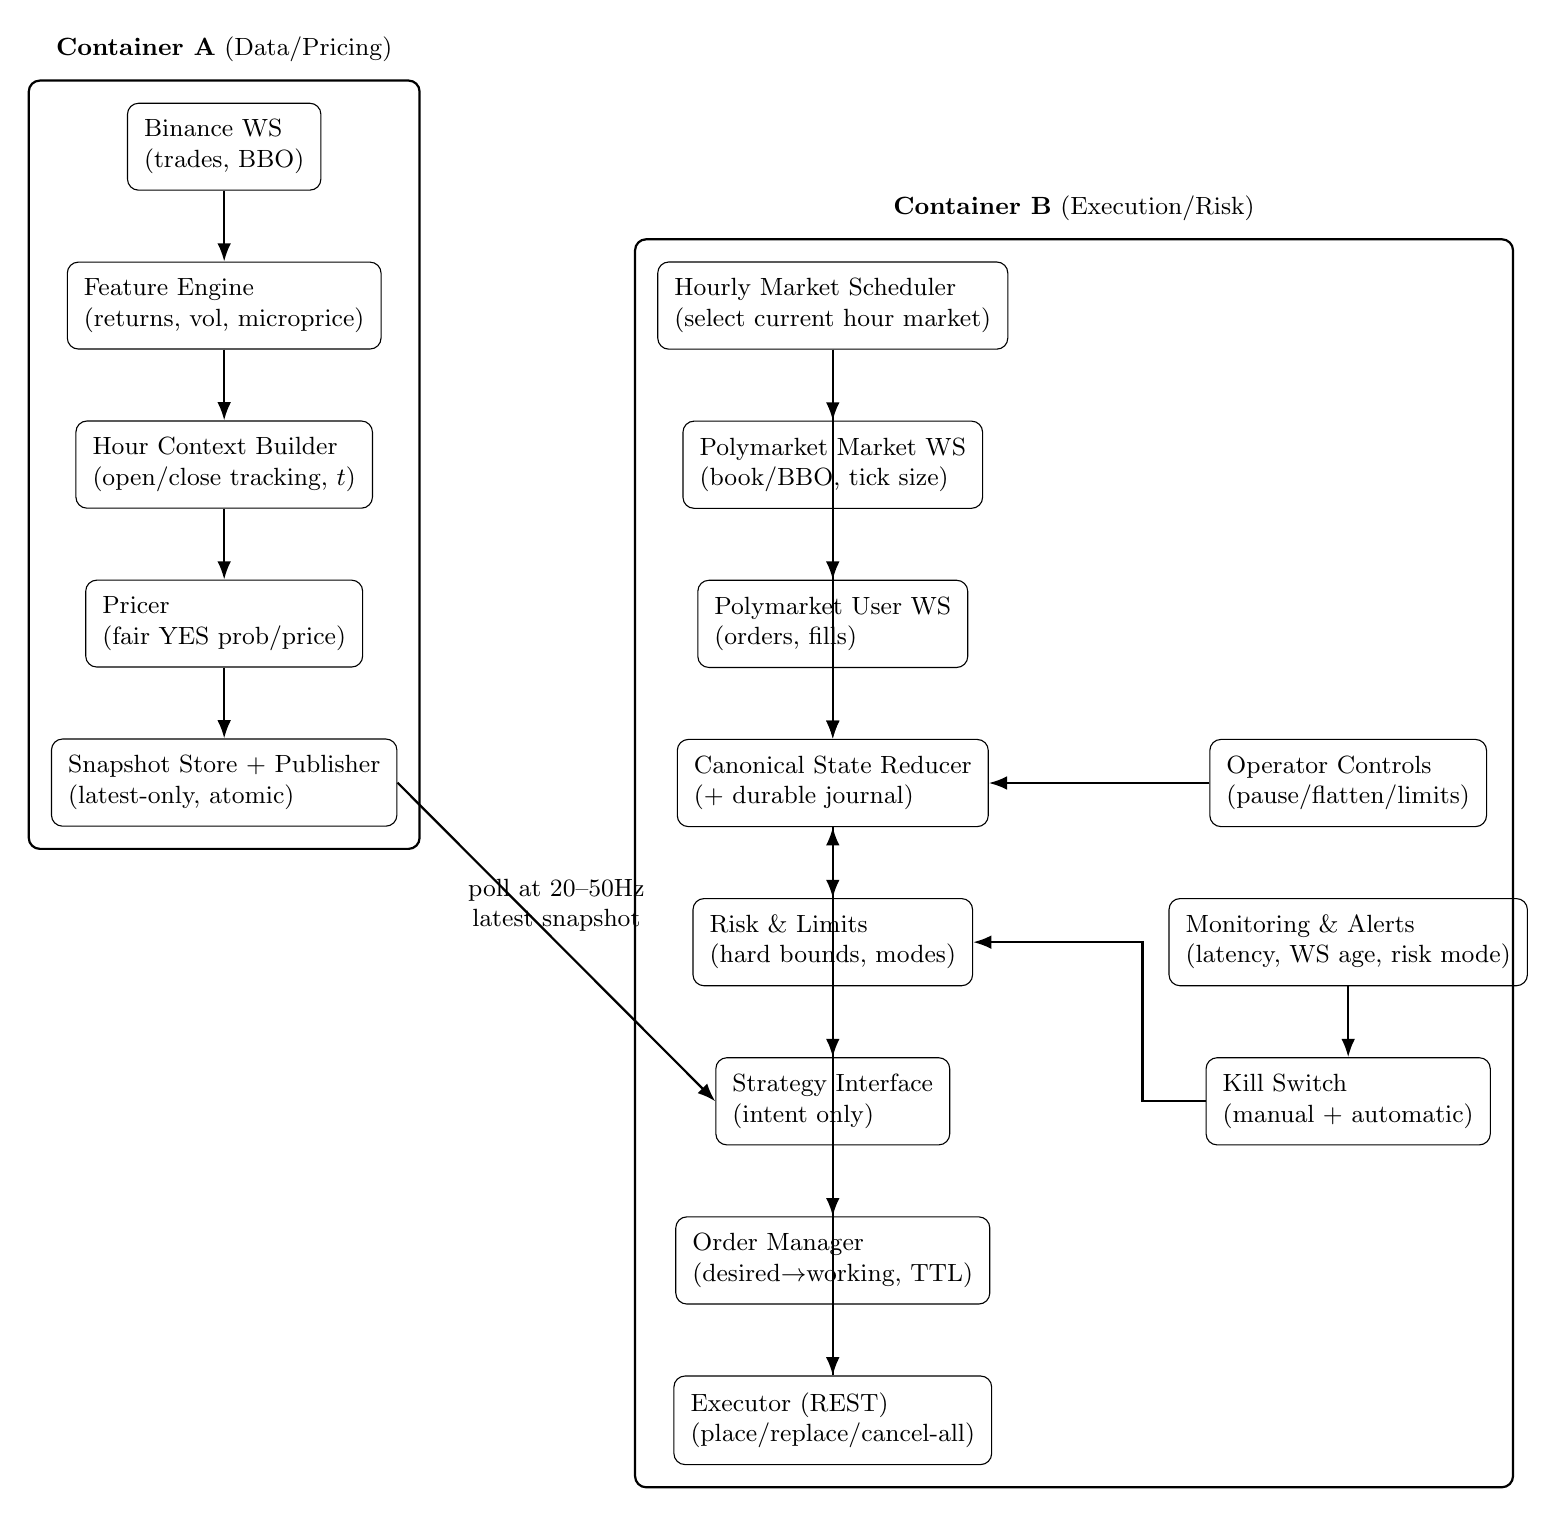
\begin{tikzpicture}[
  font=\small,
  box/.style={draw, rounded corners, align=left, inner sep=6pt},
  arrow/.style={-Latex, thick},
  node distance=9mm and 12mm
]

% Container A nodes
\node[box] (binws) {Binance WS\\(trades, BBO)};
\node[box, below=of binws] (feat) {Feature Engine\\(returns, vol, microprice)};
\node[box, below=of feat] (hourctx) {Hour Context Builder\\(open/close tracking, $t$)};
\node[box, below=of hourctx] (pricer) {Pricer\\(fair YES prob/price)};
\node[box, below=of pricer] (snap) {Snapshot Store + Publisher\\(latest-only, atomic)};

\draw[arrow] (binws) -- (feat);
\draw[arrow] (feat) -- (hourctx);
\draw[arrow] (hourctx) -- (pricer);
\draw[arrow] (pricer) -- (snap);

\node[draw, thick, rounded corners, fit=(binws)(snap), inner sep=8pt, label={[yshift=1mm]\containerA}] (Abox) {};

% Container B nodes
\node[box, right=35mm of feat] (sched) {Hourly Market Scheduler\\(select current hour market)};
\node[box, below=of sched] (pmktm) {Polymarket Market WS\\(book/BBO, tick size)};
\node[box, below=of pmktm] (pmktu) {Polymarket User WS\\(orders, fills)};
\node[box, below=of pmktu] (reducer) {Canonical State Reducer\\(+ durable journal)};
\node[box, below=of reducer] (risk) {Risk \& Limits\\(hard bounds, modes)};
\node[box, below=of risk] (strategy) {Strategy Interface\\(intent only)};
\node[box, below=of strategy] (om) {Order Manager\\(desired$\to$working, TTL)};
\node[box, below=of om] (exec) {Executor (REST)\\(place/replace/cancel-all)};
\node[box, right=28mm of reducer] (ctrl) {Operator Controls\\(pause/flatten/limits)};
\node[box, below=of ctrl] (mon) {Monitoring \& Alerts\\(latency, WS age, risk mode)};
\node[box, below=of mon] (ks) {Kill Switch\\(manual + automatic)};

\draw[arrow] (sched) -- (pmktm);
\draw[arrow] (sched) -- (pmktu);
\draw[arrow] (pmktm) -- (reducer);
\draw[arrow] (pmktu) -- (reducer);
\draw[arrow] (ctrl) -- (reducer);
\draw[arrow] (reducer) -- (risk);
\draw[arrow] (risk) -- (strategy);
\draw[arrow] (strategy) -- (om);
\draw[arrow] (om) -- (exec);
\draw[arrow] (exec) -- (reducer);

\draw[arrow] (mon) -- (ks);
\draw[arrow] (ks.west) -- ++(-8mm,0) |- (risk.east);

\node[draw, thick, rounded corners, fit=(sched)(exec)(ctrl)(ks), inner sep=8pt, label={[yshift=1mm]\containerB}] (Bbox) {};

% Inter-container polling arrow
\draw[arrow] (snap.east) -- node[above, align=center]{poll at 20--50Hz\\latest snapshot} (strategy.west);

\end{tikzpicture}
\caption{Two-container architecture. Container A publishes an atomic ``latest snapshot''. Container B samples it on a fixed-frequency decision loop and enforces risk, state correctness, and execution safety.}
\end{figure}

% ============================================================
\section{Container A: Data/Pricing (Binance)}

\subsection{Responsibilities}
\containerA\ is designed for high-frequency streaming ingestion and feature computation. It is \textbf{not} allowed to:
\begin{itemize}[leftmargin=*, itemsep=2pt]
  \item place orders,
  \item maintain Polymarket positions,
  \item decide trading actions.
\end{itemize}
It \textbf{must}:
\begin{itemize}[leftmargin=*, itemsep=2pt]
  \item maintain the most recent Binance market state (trades, BBO),
  \item compute rolling features (volatility estimates, returns, microstructure signals),
  \item compute the hour context (open price, $t_\text{remaining}$),
  \item produce a fair value estimate for the current hourly Polymarket market,
  \item publish a single atomic snapshot that can be read at any time.
\end{itemize}

\subsection{Event Time vs Receive Time}
Every ingested event carries:
\begin{itemize}[leftmargin=*, itemsep=2pt]
  \item \textbf{Exchange timestamp} (event time) from Binance,
  \item \textbf{Local receive timestamp} (when the system observed it).
\end{itemize}
Design requirement: feature computations are anchored to exchange time as much as possible, but staleness detection uses local receive time.

\subsection{Hour Context and Reference Construction}
The Hour Context Builder maintains:
\begin{itemize}[leftmargin=*, itemsep=2pt]
  \item \texttt{hour\_id}, \texttt{hour\_start\_ts}, \texttt{hour\_end\_ts},
  \item \texttt{open\_price} for the hour (once set, immutable),
  \item \texttt{last\_trade\_price} observed and its exchange timestamp,
  \item time-to-end \texttt{t\_remaining\_ms}.
\end{itemize}
When the system crosses into a new hour:
\begin{itemize}[leftmargin=*, itemsep=2pt]
  \item a new \texttt{hour\_id} is created,
  \item \texttt{open\_price} is reset and set by the first qualifying trade,
  \item feature windows that depend on hour boundaries are reset or rolled according to configuration.
\end{itemize}

\subsection{Pricer Output Contract}
The Pricer transforms features into a probability (and optionally uncertainty) used by strategies:
\begin{itemize}[leftmargin=*, itemsep=2pt]
  \item \texttt{p\_yes\_fair} $\in [0,1]$ (interpretable as a fair Polymarket price),
  \item \texttt{p\_yes\_band} (e.g., lower/upper bound or one-sigma),
  \item optional: \texttt{recommended\_spread\_ticks}, \texttt{edge\_threshold\_ticks}.
\end{itemize}
The pricer is a \textbf{pluggable component}: multiple pricing models can be swapped without changing execution or risk.

\subsection{Snapshot Publisher Semantics (Latest-Only Pull)}
Container A exposes a \emph{latest-only} snapshot interface that guarantees:
\begin{itemize}[leftmargin=*, itemsep=2pt]
  \item \textbf{Atomicity}: each read returns a self-consistent snapshot (no partial updates).
  \item \textbf{Monotonic sequence}: \texttt{seq} increases by 1 for each published snapshot.
  \item \textbf{Staleness flags}: snapshot includes \texttt{age\_ms} and \texttt{stale} derived from last Binance event receive time.
  \item \textbf{Bounded size}: snapshot is compact and bounded to avoid backpressure or memory growth.
\end{itemize}
This design prevents the execution loop from depending on high-rate event streams and provides clean failure semantics (stale data is explicit).

% ============================================================
\section{Container B: Execution/Risk (Polymarket)}

\subsection{Responsibilities}
\containerB\ owns all financially dangerous state and actions. It must:
\begin{itemize}[leftmargin=*, itemsep=2pt]
  \item track Polymarket market state (book/BBO, tick size changes),
  \item track user state (orders, fills, positions, capital),
  \item enforce hard risk limits and safe modes,
  \item run the decision loop and apply strategy intents,
  \item place/replace/cancel orders via a disciplined order manager,
  \item provide operator controls and monitoring.
\end{itemize}

\subsection{Market Scheduler (Hourly Specialization)}
The Market Scheduler selects the current active hour market and its identifiers:
\begin{itemize}[leftmargin=*, itemsep=2pt]
  \item \texttt{condition\_id} for the hour market,
  \item token identifiers for YES/NO,
  \item market close time and operational status.
\end{itemize}
Design requirement: only one market is active at a time. On hour rollover, the system transitions to the next market using an explicit session state machine (Section~\ref{sec:session-sm}).

\subsection{Connectivity Model}
Container B maintains independent health states for:
\begin{itemize}[leftmargin=*, itemsep=2pt]
  \item Polymarket Market websocket (public market updates),
  \item Polymarket User websocket (authenticated user events),
  \item Polymarket REST execution endpoint,
  \item Binance snapshot freshness (indirect via Container A snapshot).
\end{itemize}
Each health state is mapped into a \textbf{risk mode} that gates allowed actions (Section~\ref{sec:risk}).

% ============================================================
\section{Canonical State, Event Sourcing, and Persistence}

\subsection{Single-Writer Canonical State Reducer}
The core safety invariant is:

\begin{quote}
\textbf{Invariant S1 (Single Writer):} A single canonical state reducer is the only component allowed to mutate trading state (positions, open orders, reserved capital, modes).
\end{quote}

All external and internal events are serialized through the reducer. This yields deterministic behavior, avoids race conditions, and ensures operator commands are auditable.

\subsection{Durable Journal and Snapshots}
Because websockets provide ``now'' rather than history, the system maintains a durable local journal in SQLite (WAL recommended):
\begin{itemize}[leftmargin=*, itemsep=2pt]
  \item \textbf{Journal entries}: every inbound websocket message (market+user), every outbound REST request intent, every REST response/exception, and every operator command.
  \item \textbf{State snapshots}: periodic snapshots of the reduced canonical state to enable fast restart.
\end{itemize}

\subsection{Restart Semantics}
On restart, the system:
\begin{itemize}[leftmargin=*, itemsep=2pt]
  \item reconstructs the latest canonical state from the most recent snapshot + journal tail,
  \item reconnects websockets,
  \item performs a \textbf{conservative reconciliation} cycle (Section~\ref{sec:recon}),
  \item remains in a conservative risk mode until order/position state is known-good.
\end{itemize}

% ============================================================
\section{Decision Loop and Strategy Interface}

\subsection{Fixed-Frequency Decision Tick}
The decision loop runs at a fixed frequency (e.g., 20--50Hz). Each tick reads:
\begin{enumerate}[leftmargin=*, itemsep=2pt]
  \item the latest Binance snapshot from Container A,
  \item the latest Polymarket market view (BBO/tick size),
  \item the canonical internal state (positions, open orders, mode, time remaining).
\end{enumerate}
The loop produces \textbf{strategy intent} that is then filtered by risk and translated into order-manager actions.

\subsection{Strategy Contract (Intent Only)}
A strategy is restricted to output:
\begin{itemize}[leftmargin=*, itemsep=2pt]
  \item up to one (optionally two) desired quote orders per side (price, size, expiration horizon),
  \item optional taker actions (marketable orders) only when permitted by risk mode,
  \item an optional target inventory or skew request.
\end{itemize}

\textbf{Prohibition:} the strategy does not call execution endpoints directly and cannot bypass the order manager or risk engine.

\subsection{Opportunistic Quoting}
The default posture is \emph{opportunistic}:
\begin{itemize}[leftmargin=*, itemsep=2pt]
  \item If the estimated edge is below threshold, the desired quote set is empty (no orders).
  \item If edge exists, the system posts limited, time-bombed quotes (Section~\ref{sec:orders}).
  \item Quote churn is minimized due to RTT constraints; replacements occur only when meaningful.
\end{itemize}

% ============================================================
\section{Order Lifecycle, Idempotency, and Quote Safety}
\label{sec:orders}

\subsection{Desired-State Reconciliation}
The order manager operates as:
\[
\text{desired orders} \longrightarrow \text{reconcile with working orders} \longrightarrow \text{actions (place/replace/cancel)}.
\]
This ensures that the system converges toward the desired state even under partial fills, missed acks, or retries.

\subsection{Time-Bombed Quotes (Expiration / TTL)}
All quotes are placed with explicit expiration (GTD-style). This provides a hard safety guarantee:

\begin{quote}
\textbf{Invariant O1 (No Indefinite Orders):} No order may remain live beyond a bounded horizon, even if the system disconnects.
\end{quote}

Expiration horizons are linked to:
\begin{itemize}[leftmargin=*, itemsep=2pt]
  \item decision refresh rate (orders expire within a small multiple of the update period),
  \item the session phase (orders expire sooner as the hour end approaches),
  \item operator mode (reduce-only and flatten modes shorten or eliminate quote lifetimes).
\end{itemize}

\subsection{Replace vs Cancel-and-Place}
Order updates are governed by explicit rules:
\begin{itemize}[leftmargin=*, itemsep=2pt]
  \item Replace only if price moves by at least \texttt{replace\_min\_ticks} or size changes beyond \texttt{replace\_min\_size}.
  \item Otherwise keep the working order to reduce churn and avoid self-induced adverse selection.
  \item When tick size changes, re-round and reconcile all working quotes.
\end{itemize}

\subsection{Unknown Order State}
If the system submits an order but cannot confirm its status (e.g., REST timeout, websocket gap):
\begin{itemize}[leftmargin=*, itemsep=2pt]
  \item the order is marked \texttt{UNKNOWN},
  \item the system transitions to a conservative mode (REDUCE\_ONLY or HALT depending on severity),
  \item upon connectivity restoration: \textbf{cancel-all} then rebuild from user events.
\end{itemize}

\subsection{Cancel-All-on-Reconnect}
Because disconnects are treated as emergency events, the system uses a standardized reconnect sequence:
\begin{enumerate}[leftmargin=*, itemsep=2pt]
  \item Reconnect websockets.
  \item Immediately issue cancel-all for the active market.
  \item Stop all new risk-taking until cancellation is confirmed or a safety timeout is reached.
  \item Resume only after a clean state is achieved (no live orders, stable user stream).
\end{enumerate}

% ============================================================
\section{Risk, Limits, and Safety Modes}
\label{sec:risk}

\subsection{Hard Limits}
Hard limits are \emph{always} enforced, regardless of strategy:
\begin{itemize}[leftmargin=*, itemsep=2pt]
  \item Max capital per hour market (filled + reserved).
  \item Max position size (YES and NO) and/or net exposure.
  \item Max number of open orders.
  \item Max order size.
  \item Max order rate (placements and cancels per second).
  \item Max tolerated staleness of Binance snapshot.
\end{itemize}

\subsection{Reserved Capital Model}
The risk engine computes:
\[
\texttt{reserved\_capital} = \texttt{capital\_used\_by\_filled\_positions} + \texttt{worst\_case\_capital\_needed\_for\_open\_orders}.
\]
This model is explicitly conservative. It must treat each open order as fully fillable at any time, and reserve collateral accordingly. The conservatism level is configurable.

\subsection{Session-Phase Inventory Decay}
To free capital before hour end, the risk framework defines a time-dependent target inventory:
\[
\texttt{target\_inventory}(t) \rightarrow 0 \quad \text{as } t \to \texttt{hour\_end}.
\]
As time remaining decreases:
\begin{itemize}[leftmargin=*, itemsep=2pt]
  \item allowed inventory is reduced,
  \item opening new exposure requires higher edge,
  \item quote sizes are automatically scaled down,
  \item liquidation bias increases (skew to unwind).
\end{itemize}

\subsection{Risk Modes}
The system uses modes that gate allowed actions:
\begin{center}
\begin{tabular}{@{}p{0.22\linewidth}p{0.73\linewidth}@{}}
\toprule
\textbf{Mode} & \textbf{Allowed Actions} \\
\midrule
NORMAL & Quoting and taking allowed within limits. \\
REDUCE\_ONLY & Only actions that reduce worst-case exposure. No new risk. Quotes may be posted only if they strictly unwind inventory. \\
FLATTEN & Aggressive reduction toward zero inventory. Cancels exposure-increasing orders. Allows only unwind intents. \\
HALT & No new orders. Cancel-all is permitted. Used for severe uncertainty (WS down, unknown state). \\
\bottomrule
\end{tabular}
\end{center}

\subsection{Circuit Breakers}
Automatic circuit breakers trigger mode transitions based on:
\begin{itemize}[leftmargin=*, itemsep=2pt]
  \item Binance snapshot staleness beyond threshold,
  \item Polymarket websocket disconnection or prolonged silence,
  \item repeated REST failures or rate-limit signals,
  \item internal loop lag beyond threshold,
  \item anomalous state divergence (e.g., negative reserved capital, impossible fills).
\end{itemize}

% ============================================================
\section{Hourly Session State Machine}
\label{sec:session-sm}

\subsection{Session States}
The hourly lifecycle is explicit:
\begin{enumerate}[leftmargin=*, itemsep=2pt]
  \item \textbf{BOOT\_SYNC}: connect streams, cancel-all, establish clean start.
  \item \textbf{ACTIVE}: normal opportunistic trading.
  \item \textbf{WIND\_DOWN}: gradually reduce inventory targets; restrict new exposure.
  \item \textbf{FLATTEN}: enforce exit; prefer being flat before hour end.
  \item \textbf{DONE}: stop trading this market; transition to next hour market.
\end{enumerate}

\subsection{State Diagram}
\begin{figure}[h]
\centering
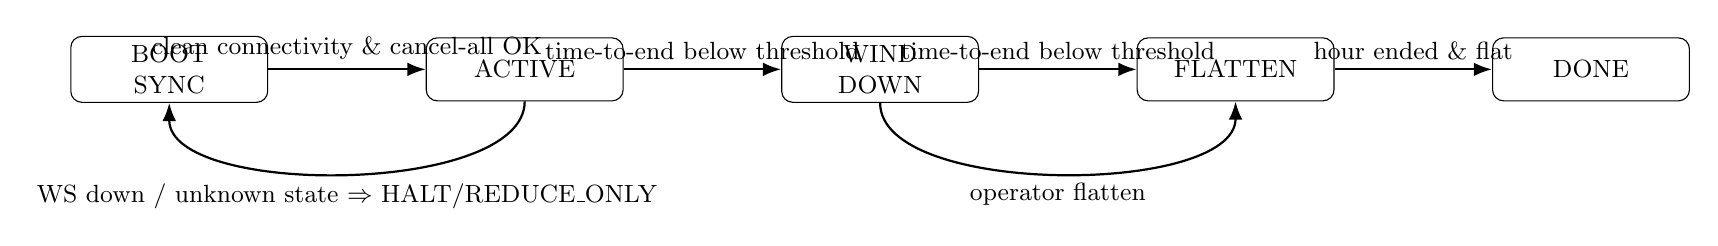
\begin{tikzpicture}[
  node distance=20mm,
  every node/.style={font=\small},
  state/.style={draw, rounded corners, minimum width=25mm, minimum height=8mm, align=center},
  arrow/.style={-Latex, thick}
]
\node[state] (boot) {BOOT\\SYNC};
\node[state, right=of boot] (active) {ACTIVE};
\node[state, right=of active] (wind) {WIND\\DOWN};
\node[state, right=of wind] (flat) {FLATTEN};
\node[state, right=of flat] (done) {DONE};

\draw[arrow] (boot) -- node[above]{clean connectivity \& cancel-all OK} (active);
\draw[arrow] (active) -- node[above]{time-to-end below threshold} (wind);
\draw[arrow] (wind) -- node[above]{time-to-end below threshold} (flat);
\draw[arrow] (flat) -- node[above]{hour ended \& flat} (done);

\draw[arrow] (active.south) .. controls +(0,-12mm) and +(0,-12mm) .. node[below]{WS down / unknown state $\Rightarrow$ HALT/REDUCE\_ONLY} (boot.south);
\draw[arrow] (wind.south) .. controls +(0,-12mm) and +(0,-12mm) .. node[below]{operator flatten} (flat.south);

\end{tikzpicture}
\caption{Hourly session state machine. Risk modes (NORMAL/REDUCE\_ONLY/HALT) can be active \emph{within} a session state; session states control time-based behavior and market selection.}
\end{figure}

\subsection{Transition Table (Operational)}
\begin{longtable}{@{}p{0.18\linewidth}p{0.28\linewidth}p{0.48\linewidth}@{}}
\toprule
\textbf{From} & \textbf{Trigger} & \textbf{To / Action} \\
\midrule
BOOT\_SYNC & WS connected + cancel-all issued & Stay BOOT\_SYNC until safe; no trading \\
BOOT\_SYNC & No live orders + user stream stable & ACTIVE \\
ACTIVE & $t_\text{remaining} \le T_\text{wind}$ & WIND\_DOWN \\
WIND\_DOWN & $t_\text{remaining} \le T_\text{flatten}$ & FLATTEN \\
ANY & Polymarket WS down / silence & HALT mode + reconnect + cancel-all \\
ANY & Binance stale beyond threshold & REDUCE\_ONLY mode \\
ANY & Operator \texttt{flatten\_now} & FLATTEN + REDUCE\_ONLY \\
FLATTEN & hour ended and flat & DONE \\
DONE & next market discovered & BOOT\_SYNC (next hour) \\
\bottomrule
\end{longtable}

% ============================================================
\section{Reconciliation, Consistency, and Correctness}
\label{sec:recon}

\subsection{Why Reconciliation Exists}
Even if websockets are the preferred source of truth, the system must handle:
\begin{itemize}[leftmargin=*, itemsep=2pt]
  \item missed websocket messages,
  \item duplicate messages,
  \item ordering anomalies across channels,
  \item REST timeouts and unknown acknowledgements.
\end{itemize}

\subsection{Reconciliation Policy}
Reconciliation is deliberately conservative and simple:
\begin{enumerate}[leftmargin=*, itemsep=2pt]
  \item \textbf{Cancel-all} on reconnect or uncertainty.
  \item Treat any uncertain state as \textbf{HALT} or \textbf{REDUCE\_ONLY}.
  \item Require a stabilization window (e.g., consecutive healthy ticks) before resuming NORMAL trading.
\end{enumerate}

\subsection{Tick Size Changes}
Tick size changes can occur (e.g., near extreme prices). The system treats tick size as a dynamic market parameter:
\begin{itemize}[leftmargin=*, itemsep=2pt]
  \item All desired prices are rounded using the latest tick size.
  \item On tick change, the order manager re-evaluates and reconciles all working quotes.
\end{itemize}

% ============================================================
\section{Failure Modes and Safe Responses}

\subsection{Binance Websocket Disconnect}
Symptoms:
\begin{itemize}[leftmargin=*, itemsep=2pt]
  \item Container A snapshot \texttt{age\_ms} increases and \texttt{stale=true}.
\end{itemize}
Response:
\begin{itemize}[leftmargin=*, itemsep=2pt]
  \item Container B transitions to REDUCE\_ONLY.
  \item No new exposure is opened.
  \item Existing inventory is unwound gracefully with passive orders (no forced market orders by default).
  \item If freshness returns quickly and remains stable, NORMAL may resume.
\end{itemize}

\subsection{Polymarket Websocket Disconnect (Emergency)}
Response:
\begin{itemize}[leftmargin=*, itemsep=2pt]
  \item Immediate HALT: no new orders.
  \item Operator notification.
  \item Reconnect attempts with backoff.
  \item Upon reconnect: cancel-all, rebuild local state, remain conservative until stabilized.
\end{itemize}
Note: GTD expirations bound risk even during outages.

\subsection{REST Failures / Rate Limits}
Response:
\begin{itemize}[leftmargin=*, itemsep=2pt]
  \item Escalate risk mode based on failure count and recency.
  \item Freeze order churn under repeated failures.
  \item Prefer cancel-all over uncertain replace storms.
\end{itemize}

\subsection{Loop Lag / Internal Backpressure}
If the decision loop cannot meet its frequency target:
\begin{itemize}[leftmargin=*, itemsep=2pt]
  \item treat as degraded state,
  \item reduce order churn,
  \item potentially transition to REDUCE\_ONLY if lag exceeds a hard threshold.
\end{itemize}

% ============================================================
\section{Operator Controls and Kill Switch}

\subsection{Control Plane Goals}
Operators must be able to safely intervene without manually trading. Controls include:
\begin{itemize}[leftmargin=*, itemsep=2pt]
  \item Pause quoting (keep risk reduction allowed),
  \item Force REDUCE\_ONLY,
  \item Force FLATTEN\_NOW,
  \item Adjust limits (max capital, max size, thresholds),
  \item Disable taker actions while allowing passive unwind.
\end{itemize}

\subsection{Kill Switch}
The kill switch is a last resort but is still designed to be \emph{orderly}:
\begin{itemize}[leftmargin=*, itemsep=2pt]
  \item Cancel-all is issued immediately.
  \item The system remains in HALT until operator clears it.
  \item Journal records the action and triggering condition.
\end{itemize}

% ============================================================
\section{Observability, Auditability, and PnL}

\subsection{Metrics}
Key metrics (minimum set):
\begin{itemize}[leftmargin=*, itemsep=2pt]
  \item Websocket last-message age (market and user streams),
  \item Binance snapshot staleness and sequence gaps,
  \item Decision-loop lag and tick rate,
  \item Order round-trip latency (submit $\to$ visible in state),
  \item Open order count, position size, reserved capital, active mode/state.
\end{itemize}

\subsection{Logging and Audit}
All decisions and external interactions are recorded:
\begin{itemize}[leftmargin=*, itemsep=2pt]
  \item structured logs for human debugging,
  \item durable SQLite journal for post-mortems and exact replay.
\end{itemize}

\subsection{PnL Model}
Intrahour PnL is approximate:
\begin{itemize}[leftmargin=*, itemsep=2pt]
  \item mark-to-market uses current mid prices (or fair estimates) for YES/NO,
  \item realized PnL is finalized at market resolution based on token payouts,
  \item risk decisions do not depend on the precision of intrahour PnL.
\end{itemize}

% ============================================================
\section{Extensibility (Within a Specialized Framework)}

\subsection{Swap-in Pricing Models}
Container A supports multiple pricer variants producing the same snapshot contract. Container B remains unchanged.

\subsection{Swap-in Strategies}
Strategies can be swapped provided they adhere to the intent-only contract and accept that risk modes and session phases may override or nullify their intents.

\subsection{Future: Multiple Hour Markets}
The design can generalize to multiple simultaneous markets by:
\begin{itemize}[leftmargin=*, itemsep=2pt]
  \item turning the canonical reducer into a per-market shard,
  \item preserving single-writer per shard,
  \item applying portfolio-level risk above the shards.
\end{itemize}
This is explicitly out of scope for the current system.

% ============================================================
\appendix
\section{Appendix A: Data Contracts (Schemas)}

\subsection{A.1 Binance Snapshot (Container A $\to$ Container B)}
\begin{longtable}{@{}p{0.22\linewidth}p{0.14\linewidth}p{0.56\linewidth}@{}}
\toprule
\textbf{Field} & \textbf{Type} & \textbf{Meaning / Invariants} \\
\midrule
\texttt{seq} & int & Monotonic sequence for snapshots; increments on publish. \\
\texttt{ts\_local\_ms} & int & Local time of snapshot creation (monotonic reference for age). \\
\texttt{ts\_exchange\_ms} & int & Exchange event time of last incorporated Binance event. \\
\texttt{age\_ms} & int & Now - last Binance event receive time (local). \\
\texttt{stale} & bool & True if \texttt{age\_ms} exceeds configured threshold. \\
\texttt{hour\_id} & string & UTC hour identifier (e.g., 2026-01-22T14:00:00Z). \\
\texttt{hour\_start\_ts} & int & Hour start in epoch ms (UTC). \\
\texttt{hour\_end\_ts} & int & Hour end in epoch ms (UTC). \\
\texttt{t\_remaining\_ms} & int & Time remaining to hour end (>=0). \\
\texttt{open\_price} & float & Hour open reference; immutable once set. \\
\texttt{last\_trade\_price} & float & Latest trade price. \\
\texttt{bbo\_bid} / \texttt{bbo\_ask} & float & Latest best bid/ask. \\
\texttt{mid} & float & Derived mid price. \\
\texttt{vol\_realized\_x} & float & One or more realized vol estimates (windows configurable). \\
\texttt{p\_yes\_fair} & float & Fair YES price/probability in [0,1]. \\
\texttt{p\_yes\_band\_lo/hi} & float & Optional uncertainty bounds. \\
\bottomrule
\end{longtable}

\subsection{A.2 Polymarket Market View (Internal to Container B)}
\begin{longtable}{@{}p{0.22\linewidth}p{0.14\linewidth}p{0.56\linewidth}@{}}
\toprule
\textbf{Field} & \textbf{Type} & \textbf{Meaning / Invariants} \\
\midrule
\texttt{market\_id} & string & Identifier for current hour market. \\
\texttt{tick\_size} & float & Current tick size, dynamic. \\
\texttt{best\_bid} / \texttt{best\_ask} & float & Current BBO in [0,1]. \\
\texttt{book\_ts\_local\_ms} & int & Local time last market update was received. \\
\texttt{ws\_age\_ms} & int & Age since last market WS message. \\
\bottomrule
\end{longtable}

\subsection{A.3 Canonical Trading State (Reducer-Owned)}
\begin{longtable}{@{}p{0.22\linewidth}p{0.14\linewidth}p{0.56\linewidth}@{}}
\toprule
\textbf{Field} & \textbf{Type} & \textbf{Meaning / Invariants} \\
\midrule
\texttt{session\_state} & enum & BOOT\_SYNC / ACTIVE / WIND\_DOWN / FLATTEN / DONE \\
\texttt{risk\_mode} & enum & NORMAL / REDUCE\_ONLY / FLATTEN / HALT \\
\texttt{pos\_yes} / \texttt{pos\_no} & float & Current token holdings (can be fractional). \\
\texttt{open\_orders} & map & All working orders with status and timestamps. \\
\texttt{reserved\_capital} & float & Conservative bound of capital usage. \\
\texttt{health} & struct & WS ages, REST health, stale flags. \\
\texttt{limits} & struct & Current configured limits (operator-adjustable). \\
\bottomrule
\end{longtable}

\subsection{A.4 Order Intent (Strategy Output)}
\begin{longtable}{@{}p{0.22\linewidth}p{0.14\linewidth}p{0.56\linewidth}@{}}
\toprule
\textbf{Field} & \textbf{Type} & \textbf{Meaning / Invariants} \\
\midrule
\texttt{side} & enum & BUY\_YES / SELL\_YES / BUY\_NO / SELL\_NO (depending on venue semantics) \\
\texttt{price} & float & Must be rounded to tick size and in [0,1]. \\
\texttt{size} & float & Must be within max order size; may be scaled by risk. \\
\texttt{expires\_at\_ms} & int & Explicit expiration (time-bomb). \\
\texttt{purpose} & enum & QUOTE / UNWIND / TAKE \\
\bottomrule
\end{longtable}

\subsection{A.5 Operator Commands}
\begin{longtable}{@{}p{0.26\linewidth}p{0.68\linewidth}@{}}
\toprule
\textbf{Command} & \textbf{Semantics} \\
\midrule
\texttt{pause\_quoting=true/false} & Disable/enable new quote intents; allow unwind if needed. \\
\texttt{set\_mode=REDUCE\_ONLY/HALT} & Force risk mode. \\
\texttt{flatten\_now} & Transition session to FLATTEN and enforce unwind-only behavior. \\
\texttt{set\_limits(\dots)} & Adjust max capital, max size, thresholds, timers. \\
\bottomrule
\end{longtable}

% ============================================================
\section{Appendix B: Configuration Parameters (Recommended Starting Point)}
This appendix lists configuration \emph{dimensions} to finalize during commissioning. Exact numeric values are strategy- and capital-dependent.

\begin{itemize}[leftmargin=*, itemsep=2pt]
  \item Decision tick frequency: 20--50Hz.
  \item Binance stale threshold: e.g., 200--1000ms (tune to connection quality).
  \item Replace thresholds: minimum ticks and minimum time between replaces.
  \item Max orders: typically 0--2 working quotes per side (keep small).
  \item Session timers: $T_\text{wind}$, $T_\text{flatten}$, and a final safety cutoff.
  \item Expiration horizon: a small multiple of decision period, shrinking as $t_\text{remaining}\to 0$.
  \item Capital limits: per-market max reserved capital and per-order caps.
\end{itemize}

% ============================================================
\section{Appendix C: Safety Invariants Checklist}
\begin{enumerate}[leftmargin=*, itemsep=2pt]
  \item (S1) Single-writer reducer owns all mutable trading state.
  \item (O1) No indefinite orders: all quotes expire (GTD/TTL).
  \item Under uncertainty, system reduces risk: REDUCE\_ONLY/HALT.
  \item Cancel-all on reconnect or unknown state.
  \item Hard limits always enforced; strategy cannot bypass risk.
  \item All external interactions are journaled durably.
  \item Session states explicitly control hour rollover and end-of-hour flattening.
\end{enumerate}

% ============================================================
\section{Appendix D: Glossary}
\begin{itemize}[leftmargin=*, itemsep=2pt]
  \item \textbf{BBO}: Best bid/offer (best bid price and best ask price).
  \item \textbf{GTD}: Good-Till-Date (order expiration time is set).
  \item \textbf{RTT}: Round-trip time (submit request $\to$ observe acknowledgement/state change).
  \item \textbf{Reducer}: Single-threaded state transition function consuming serialized events.
  \item \textbf{Reserved capital}: Conservative upper bound on capital usage from positions and open orders.
\end{itemize}

\end{document}
